\chapter{Einführung}
\section{Einleitung}
\label{sec:Einleitung}
Die vorliegende Arbeit beschäftigt sich mit der Fragestellung, ob und wie ein technisch konstruiertes CAD-Modell bspw. eine Maschine, ein Auto oder wie in diesem Fall eine Windenergieanlage (WEA) in das Echtzeitsystem Unity überführt werden kann, um aus diesem Modell eine VR-Anwendung zu entwickeln.
 
Zunächst wird in Kapitel 1 die Motivation zu dieser Arbeit kurz erläutert und mit Hilfe eines fachlichen Teils zur Funktion und zum Aufbau der WEA das Thema eingeleitet. 

Weiterhin sollen in Kapitel 2 die Anwendungsbereiche von CAD-Programmen und die Möglichkeiten der 3D-Modellierung beschrieben werden. Darauf aufbauend wird auf den Transfer von CAD nach Autodesk Maya anhand des Exportformates eingegangen.

Das Kapitel 3 wird sich mit einigen Grundbegriffen der 3D-Modellierung beschäftigen. Diese Grundlagen sind essentiell für die folgende Analyse des CAD-Exports. Auch die Aufbereitung des 3D-Modells für den Import in Unity wird behandelt.

Kapitel 4 wird den Bereich um Unity abdecken. Hierzu wird das Open-Source Framework VRTK zur Erstellung einer VR-Anwendung untersucht, der Szenenaufbau in Unity beschrieben. Ferner werden die implementierten Anwendungsfälle aufgelistet und konkretisiert.

Zuletzt soll in Kapitel 5 mithilfe eines Fazits konkret auf die Optimierung des Workflows und die Automatisierung von Teilschritten der Arbeit eingegangen werden. Diese haben sich durch neue Entwicklungen ergeben, konnten aber aufgrund des Projektfortschritts und dem zusätzlichen Forschungsaufwand im Rahmen dieser Arbeit  nicht mehr untersucht werden. Auch sollen abschließend noch Vorschläge und Ideen für weitere Funktionalitäten gegeben werden.


\section{Motivation}
\label{sec:Motivation}
Ein guter Freund, ein Ingenieur aus dem Maschinenbau und leidenschaftlicher VR-Spieler, trat mit einer Idee an mich heran. Er wolle eine von ihm und seiner Firma in CAD  konstruierte Maschine gerne einmal in VR betrachten. Er wisse aber nicht wie eine solche Anwendung umzusetzen sei bzw. ob es überhaupt möglich sei. Ich schlug ihm vor, dass wir Unity als Technologie für die Laufzeit- und Entwicklungsumgebung nutzen können. Nach einer kurzen Recherche  zur Kompatibilität von CAD-Formaten und den gängigen 3D-Formaten stellten wir fest, dass ein Import von CAD-Modellen nach Unity generell möglich sein muss. Da die Firma aber wie zu erwarten der Weitergabe dieser Daten nicht zustimmte, beschlossen wir auf ein Modell aus seinem Studium zurückzugreifen. Die von ihm und seinen Kommilitonen in einem Projekt konstruierte WEA stellt eine voll funktionsfähige Windenergieanlage zur Stromerzeugung dar. Dieses Modell konnten wir mit einer Umkonvertierung des Dateiformates in eine Unity-Szene importieren. Mehrere Probleme stellten wir allerdings fest. Zum ersten wies das Modell für eine Echtzeitanwendung eine extrem hohe  Anzahl an Polygonen auf. Zum zweiten war der geometrische Grundaufbau der WEA, die sogenannte Topologie nicht geeignet um ein gutes Shading in Unity zu ermöglichen. Zum dritten wurde die WEA zu einem einzigen Objekt zusammengefasst. Es war also nicht möglich Baugruppen auszublenden, einzelnen Teilen verschiedene Shader und  Skripte zuzuweisen oder diese separat zu animieren. Die WEA für einen VR-Prototypen zu optimieren schien mir daher ein geeignetes und spannendes Thema für dieses ICW. 
Um die Thematik einzuleiten wird zunächst die Funktionsweise und der Aufbau dieser WEA werden im folgenden Unterkapitel \sieheKapitel{\hyperref[sec:FachlicherKontext]{1.3 Fachlicher Kontext}} beschrieben.




\section{Fachlicher Kontext}
\label{sec:FachlicherKontext}
Die Funktionsweise einer WEA richtet sich vor allem nach der Bauart. Aber alle Anlagen erzeugen aus Windenergie Strom. Die im Wind enthaltene Leistung überträgt sich auf den Rotor der Anlage, versetzt diesen in eine Drehbewegung und treibt den in der WEA verbauten Generator an. Es wird Windenergie umgewandelt in mechanische Rotationsenergie, welche dann in elektrische Energie umgewandelt wird. \\
Generell sind Windenergieanlagen dafür konzipiert einen optimalen Energieertrag zu liefern. Diese Anlagen sind dabei unterschiedlichen Windbedingungen ausgesetzt, weshalb diese   automatisch darauf reagieren müssen um zu einer stabilen und sicheren Stromversorgung beizutragen.\footnote{Vgl. Bundesverband WindEnergie e. V.  (2018): \textit{Funktionsweise von Windenergieanlagen}.\newline
\url{https://www.wind-energie.de/themen/anlagentechnik/funktionsweise/},\newline 
abgerufen am 20.08.2018.}  





\begin{figure}[H]
	\centering
	\captionsetup{width=0.7\textwidth}
	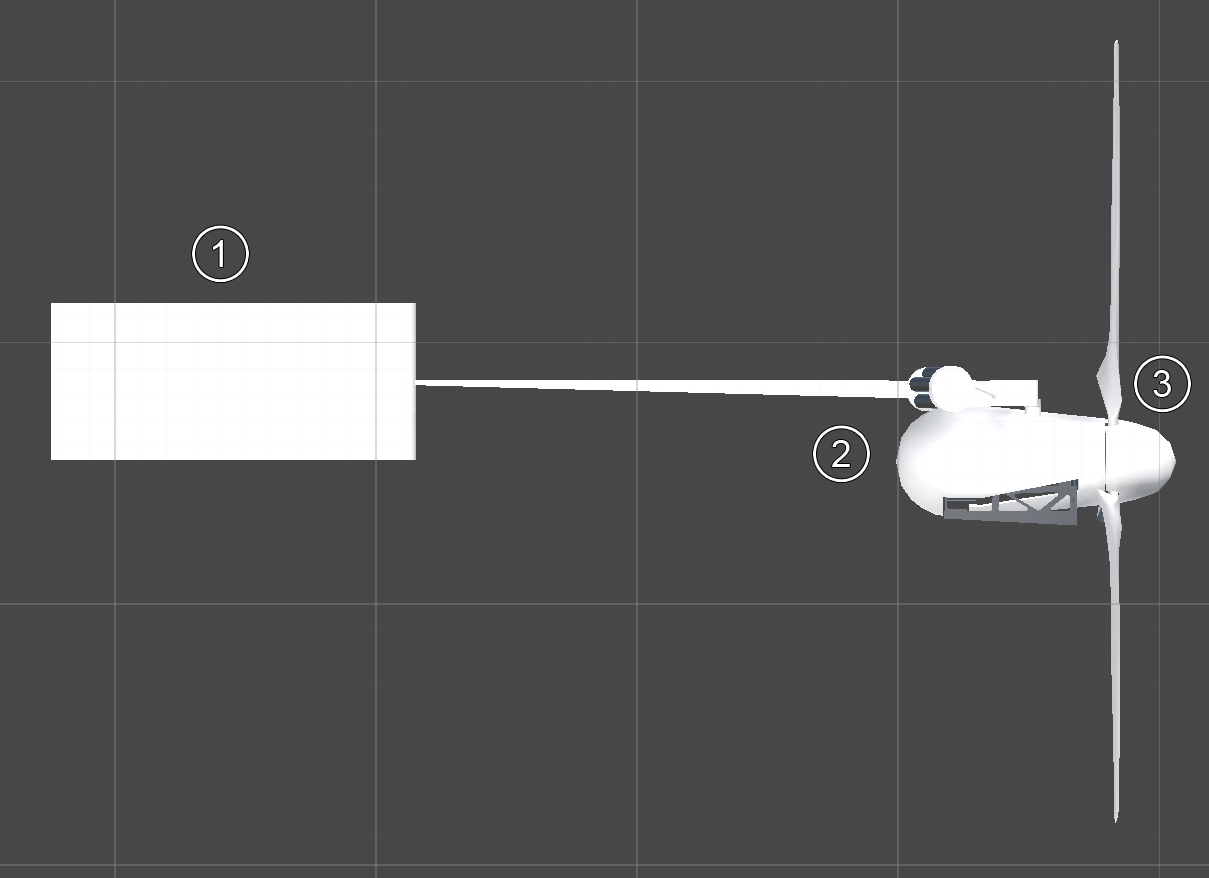
\includegraphics[keepaspectratio, width=0.7\textwidth]{bildquellen/WEA1_1}
	\caption{Äußerer Aufbau der WEA.}
	\label{fig:1}
\end{figure}

Der äußere Aufbau ist gekennzeichnet durch ein Gehäuse (die Gondel) mit montierter Windrichtungsnachführung \sieheAbbVerweis{1.1}{2}, bestehend aus einer am Windfahnenhebel angebrachten Windfahne \sieheAbbVerweis{1.1}{1}. Der Aufbau ist drehend gelagert um auch bei wechselnden Windverhältnissen einen vollautomatischen Betrieb zu gewährleisten. Ein solches Regelungssystem ist für einen zuverlässigen Betrieb unabdingbar. \\
Der Rotor, mit an der Narbe montierten Rotorblättern \sieheAbbVerweis{1.1}{3} ist nach aerodynamischen Prinzipien konstruiert und dient der Umwandlung der im Wind verfügbaren kinetischen Energie in mechanische Rotationsenergie.\footnote{Vgl. Silvio Chemnitz, Sylvio Donner, Florian Hinze, Mats Mojem, Patrick Quandt, Oliver Seidler, Moritz Will, Jens Wuthe (2013): \textit{Windpumpsysteme zur dezentralen Energieversorgung von Abwassersystemen}. TU Berlin, S. 10 ff.}

\begin{figure}[H]
	\centering
	\captionsetup{width=0.7\textwidth}
	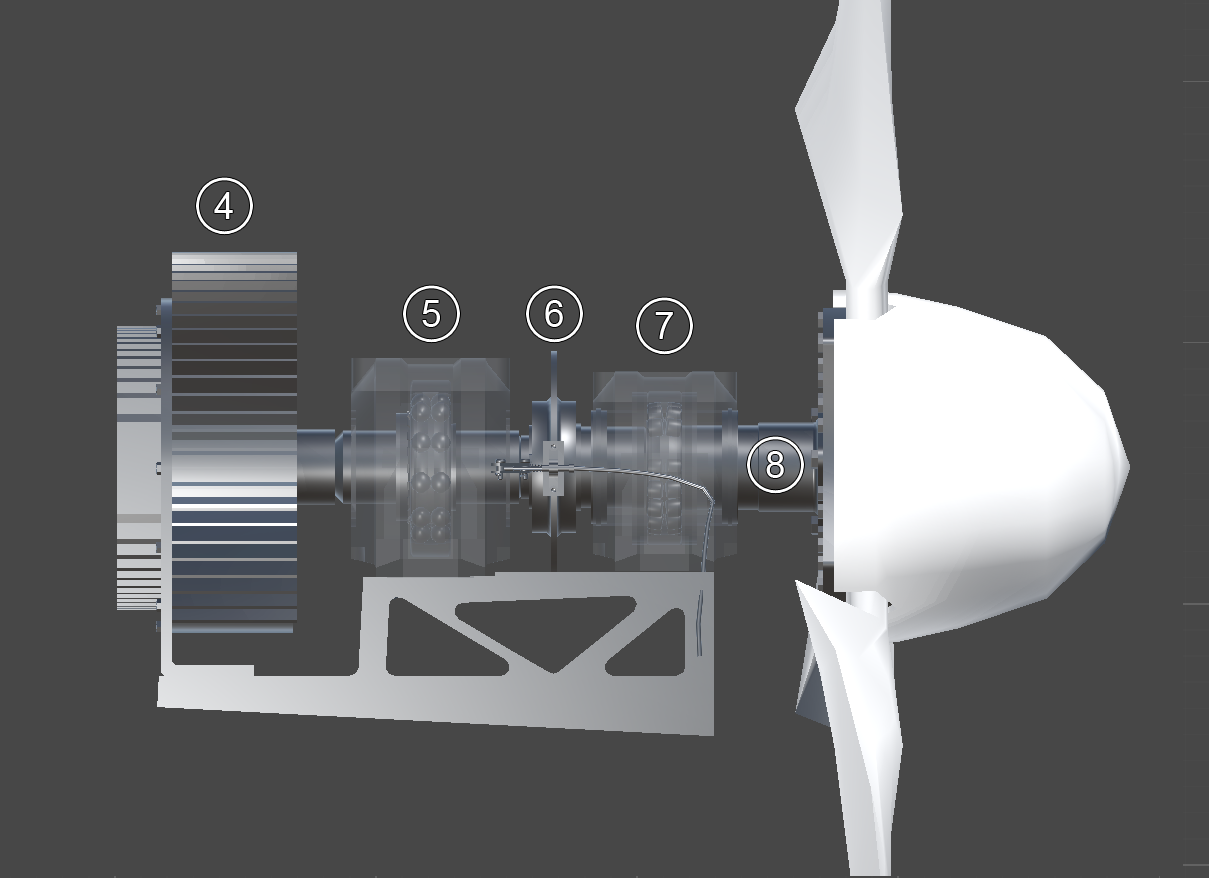
\includegraphics[keepaspectratio, width=0.7\textwidth]{bildquellen/WEA2_2}
	\caption{Innenliegende Baugruppen der WEA.}
	\label{fig:2}
\end{figure}

Für die Stromerzeugung ist ein Generator verbaut \sieheAbbVerweis{1.2}{4}. Dieser wandelt auf Basis des Induktionsgesetzes mechanische Rotationsenergie in elektrische Energie um. Es wird eine Spule in einem Magnetfeld in Rotation versetzt. Durch die Rotation wird an den Klemmen der Spule eine sinusförmige Spannung induziert.\footnote{Vgl. Prof. Dr. G. Buch, Prof. Dr. M. Krug  (2012): \textit{Kurzskriptum zur Lehrveranstaltung „Elektrische Bordnetze“ im Studiengang Fahrzeugtechnik}. Hochschule München, S. 1.1.} In diesem Beispiel erhält der Generator die verfügbare Rotationsenergie über eine Welle \sieheAbbVerweis{1.2}{8}, die über eine Kupplung mit dem Anker (Rotor) des Generators verbunden ist. Zur Kühlung während des Betriebs sind auf der Außenseite Finnen aus Aluminium angebracht.\\
Die Lagerung wird über zwei Wälzlager realisiert und als Fest-Los-Lagerung bezeichnet. Das Loslager ist ein Pendelkugellager \sieheAbbVerweis{1.2}{5} und dient zur Aufnahme der Radialkräfte, also die Kräfte, die von außen auf die Welle wirken. Als Festlager dient ein Pendelrollenlager, \sieheAbbVerweis{1.2}{7} dass die kombinierten Axial- und Radialbelastungen aufnimmt. Unter Axialkraft versteht man die Belastung die längs der Achse wirkt.
Müssen Wartungsarbeiten o.Ä. an der WEA durchgeführt werden, kann automatisches Anlaufen durch eine Bremse \sieheAbbVerweis{1.2}{6} verhindert werden. Mithilfe eines Bowdenzuges, also einem Seilzug der mechanische Kraft auf ein bewegliches Maschinenelement, in diesem Fall den Bremsbolzen überträgt, kann die WEA vom Boden aus verriegelt werden. \\
Die hier betrachtete WEA zählt zu den kleineren Modellen und hat eine Narbenhöhe von 10m. Der Turm, welcher in diesem Prototyp aus Darstellungsgründen nicht berücksichtigt wird, weist eine Höhe von 9,73m auf.\footnote{Vgl. Silvio Chemnitz, Sylvio Donner, Florian Hinze, Mats Mojem, Patrick Quandt, Oliver Seidler, Moritz Will, Jens Wuthe (2013): \textit{Windpumpsysteme zur dezentralen Energieversorgung von Abwassersystemen}. TU Berlin, S. 35--38, 44.} 
   


